%%%%%%%%%%%%%%%%%%%%%%%%%%%%%%%%%%%%%%%%%%%%%%%%%%%%%%%%%%%%%%%%%
% Dissertacao de Mestrado / Dept Fisica, CFM, UFSC              %
% Andre@UFSC - 2011                                             %
%%%%%%%%%%%%%%%%%%%%%%%%%%%%%%%%%%%%%%%%%%%%%%%%%%%%%%%%%%%%%%%%%

%:::::::::::::::::::::::::::::::::::::::::::::::::::::::::::::::%
%                                                               %
%                          Capítulo 3                           %
%                                                               %
%:::::::::::::::::::::::::::::::::::::::::::::::::::::::::::::::%

%***************************************************************%
%                                                               %
%                         Crossmatch                            %
%                                                               %
%***************************************************************%

\chapter{{\em Crossmatch} entre \SDSS/\STARLIGHT e \galex}
\label{sec:Crossmatch}


%***************************************************************%
%                                                               %
%              Crossmatch - Banco de dados do SDSS              %
%                                                               %
%***************************************************************%

\section{Banco de dados do \SDSS}

Um dos maiores responsáveis pela promoção do uso de bancos de dados relacionais
na astronomia é o projeto {\em Sloan Digital Sky Survey} (\SDSS). Inicialmente o
\SDSS utilizou um {\em sistema de gerenciamento de banco de dados orientado a
objetos} \citep{Maier1986} (OODBMS, na sigla em inglês). Após pouco mais de um
ano a abordagem se mostrou inadequada: entre os principais problemas, uma
linguagem de {\em query} inadequada e performance ruim. O motivo, segundo
\citet{Thakar2004}, foi a incapacidade da empresa desenvolvedora do OODBMS em
prover novas funcionalidades requisitadas pelo projeto e correção de {\em bugs},
bem como em acompanhar o crescimento da performance do {\em hardware}.

\subsection{Migração de OODBMS para RDBMS}
\label{sec:CrossMatch:SDSS:MigracaoRDBMS}

Todo o banco de dados do \SDSS foi migrado para um {\em sistema de gerenciamento
de banco de dados relacional} \citep{Codd1970} (RDBMS, na sigla em inglês) num
esforço guiado por \citeauthor{Thakar2004}. RDBMS pode ser considerado o padrão
da indústria. Praticamente todas as linguagens de programação tem bibliotecas de
interface às implementações de RDBMS comerciais mais comuns (Oracle, IBM e
Microsoft, Postgres). Há uma diversidade de ferramentas para desenvolvimento e
gerenciamento de RDBMS. E talvez o maior benefício de todos, o acesso aos dados
é feito utilizando uma linguagem padronizada: {\em Simple Query Language}, ou
simplesmente SQL \citep{Chamberlin1974}. A migração dos dados do \SDSS para um
RDBMS comercial implicou num aumento significativo da performance do acesso aos
dados, e resultou no desenvolvimento do {\em SkyServer}\footnote{\SDSS
SkyServer: \url{http://skyserver.sdss.org/}}. O servidor de banco de dados
escolhido pelo \SDSS foi o {\em Microsoft SQL Server}.

A comparação entre OODBMS e RDBMS no caso particular do \SDSS não implica
necessariamente a superioridade do segundo em relação ao primeiro. Tanto a
abordagem orientada a objetos quanto a abordagem relacional tem suas vantagens e
desvantagens. O estudo de caso do \SDSS é apenas uma evidência anedótica em
favor do uso de bancos de dados relacionais. No entanto, para aplicações
semelhantes ao \SDSS -- {\em surveys} astronômicos com volumes imensos de dados
-- vale a pena apostar no sucesso dos RDBMS.

\subsection{{\em SkyServer}}
\label{sec:CrossMatch:SDSS:SkyServer}

O {\em SkyServer} é um {\em website} (figura \ref{fig:TelaDoSkyServer}) que
provê acesso aos dados armazenados no banco de dados do \SDSS
\citep{Szalay2002}. O acesso mais simples pode ser feito através de um atlas de
locais famosos ({\em famous places}), que mostra imagens coloridas de objetos
celestes conhecidos. Há formulários para buscas mais sérias, gerando coleções de
imagens, espectros e tabelas de dados. No {\em SkyServer} é possível fazer
buscas avançadas utlizando SQL, embora haja limites de tempo de execução e de
quantidade de objetos retornados. Esta limitação é contornada através do sistema
{\em CasJobs}, que é tratado na seção \ref{sec:CrossMatch:SDSS:CasJobs}.

É importante ressaltar que é possível (de fato, a equipe do \SDSS encoraja)
criar {\em mirrors}\footnote{{\em Mirror}: Espelho, em inglês. Clone de um {\em
website}.} do {\em SkyServer}. Tanto o banco de dados do \SDSS quanto o código
fonte do {\em SkyServer} estão disponível no próprio {\em website} do {\em
SkyServer}. Há um clone do banco de dados do {\em Data Release} 8 do \SDSS no
servidor {\em CasJobs} do \starlight \footnote{{\em CasJobs} do \starlight:
\url{http://casjobs.starlight.ufsc.br/casjobs/}}.

\begin{figure}
	\includegraphics[width=1.0\columnwidth]{figuras/skyserver.eps}
	\caption[Telas do {\em SkyServer}.]
	{Telas do {\em SkyServer}. À esquerda, formulário para submeter uma {\em
	query} SQL. À direita, ferramenta {\em Explore} mostrando a galáxia NGC 799.}
	\label{fig:TelaDoSkyServer}
\end{figure}

\subsection{{\em CasJobs}}
\label{sec:CrossMatch:SDSS:CasJobs}

O {\em Catalog Archive Server Jobs} ({\em CasJobs}) é um serviço online
desenvolvido pela equipe do \SDSS para expandir a capacidade do {\em SkyServer}
\citep{Li2008}. Nele o usuário pode executar consultas SQL no banco de dados do
\SDSS da mesma forma que no {\em SkyServer}. Porém, além de consultas rápidas, é
possível agendar a execução de consultas mais longas. O {\em CasJobs} gerencia
estas consultas agendadas numa fila de execução, de modo a não sobrecarregar a
rede ou os servidores de banco de dados. Cada usuário possui sem próprio banco
de dados, chamado {\em MyDB}. Pode-se importar tabelas para o {\em MyDB} para
utilizar em {\em queries} correlacionando com os dados presentes no {\em
CasJobs}. O {\em MyDB} serve como armazenamento de tabelas do usuário, e há
mecanismos para exportar estas tabelas para arquivos nos formatos FITS, CSV, XML
e VOTable. Estes arquivos podem ser lidos por programas de análise de dados como
o {\em TopCat}\footnote{{\em TopCat} é um visualizador gráfico interativo e
editor de dados tabulares usado em astronomia. Ver
\url{http://www.star.bris.ac.uk/~mbt/topcat/}.}, ou mesmo importados para outros
bancos de dados.

\begin{figure}
	\includegraphics[width=0.7\columnwidth]{figuras/casjobs.eps}
	\caption[Tela do {\em CasJobs}.]
	{Tela do {\em CasJobs}. Resultado da {\em query} buscando o {\em redshift}, a
	magnitude na banda {\em g}, a cor {\em g}-{\em r} e uma amostra da imagem de
	objetos com espectroscopia.}
	\label{fig:CasJobs}
\end{figure}

É possível utilizar o {\em CasJobs} para acessar virtualmente qualquer banco de
dados. No momento, o Grupo de Astrofísica da UFSC possui um servidor {\em
CasJobs} com bancos de dados do \starlight, \SDSS DR8, GalaxyZoo\citneed, e uma
amostra do \galex e um catálogo de {\em redshifts} fotométricos
\citep{OMill2011}. O {\em CasJobs} também foi adotado por outros projetos como o
\galex, Kepler\citneed, {\em Palomar Quest}\citneed, {\em Panoramic Survey
Telescope and Rapid Response System} (Pan-STARRS) e até pelo projeto {\em
AmeriFlux}, que contém dados de hidrologia\citneed.

A figura \ref{fig:CasJobs} mostra uma tela típica de uma sessão no {\em
CasJobs}.


%***************************************************************%
%                                                               %
%          Crossmatch - Banco de dados do STARLIGHT             %
%                                                               %
%***************************************************************%

\section{Banco de dados do \STARLIGHT}

O \starlight é um código de síntese espectral \citep{CidFernandes2005}. O
programa é executado uma vez para cada galáxia do \SDSS, recebendo seu espectro
como um arquivo texto. Ele usa uma biblioteca de espectros de populações
estelares simples ({\em Single Stellar Population}, SSP)\footnote{Uma SSP
consiste num conjunto de estrelas formadas ao mesmo tempo com a mesma
metalicidade.} com diferentes idades e metalicidades como uma base do
espaço de espectros galáticos possíveis. De forma simplificada, o que o
\starlight faz é encontrar as frações de massa e luz correspondente a cada
elemento da base, ou seja, cada SSP. Analisando as relações entre os componentes
determinandos pela síntese, o programa determina diversas propriedades físicas
da galáxia, como a massa estelar total, a massa separada por idade, metalicidade
média, quantidade de poeira e velocidade de rotação, para citar apenas algumas.
Quase um milhão de espectros foram analisados, e o resultado da síntese foi
armazenado em arquivos texto.

Apenas os componentes estelares do espectro são obtidos desta forma. Subtraindo
o espectro sintetizado de luz estelar é possível medir as linhas de emissão do
espectro. Esta é uma etapa de pós-processamento, que gera um catálogo
complementar de linhas de emissão.

\subsection{Importação para o RDBMS}

Os arquivos da síntese gerados pelo \starlight ocupam uma dezena de gigabytes.
Mesmo o catálogo de propriedades físicas das galáxias, sozinho, ocupa mais de um
gigabyte. Embora seja um volume razoavelmente grande de dados, é possível
trabalhar com esta quantidade de dados num computador atual\footnote{Na época da
escrita desta dissertação, é difícil encontrar um computador novo com menos de 4
gigabytes de memória RAM.}. A transferência de arquivos com tamanho da ordem de
gigabytes pela internet também também é lugar-comum atualmente. Poderia-se
argumentar que distribuir os dados neste formato seja a forma mais adequada.

Entretanto, deve-se admitir que uma das maiores razões para o sucesso do {\em
CasJobs} em prover acesso aos dados o \SDSS não é o tamanho da base de dados, e
sim a facilidade com que o usuário pode acessar os dados e filtrar apenas o que
lhe for conveniente. Além disso, manter a base de dados num local central
permite que sejam feitas correções e revisões, o que implicaria normalmente numa
nova transferência caso cada usuário tivesse a sua cópia local.

O {\em CasJobs} requer um servidor rodando {\em Windows Server} com {\em
Internet Information Services} (IIS) e {\em Microsoft SQL Server} (MSSQL). A
instalação do {\em CasJobs} está documentada no {\em website} do {\em SkyServer}
(ver secão \ref{sec:CrossMatch:SDSS:SkyServer}). Com um servidor {\em CasJobs},
o trabalho consiste em importar os dados em arquivos texto para um banco de
dados no MSSQL. A ferramenta principal para a manipulação dos bancos de dados no
MSSQL é o {\em Microsoft SQL Server Management Studio}. Nele há um assistente
para importação de dados baseado no {\em SQL Server Integrated Services} (SSIS).
A importação das tabelas de propriedades físicas do \starlight é trivial. A
importação das linhas de emissão requer um trabalho extra para normalizar a
tabela\footnote{A normalização consiste em decompor uma tabela em tabelas
menores (com menos campos) de forma que elas fiquem melhor estruturadas. No caso
das linhas de emissão, a tabela passa de ``todas as linhas de um dado objeto num
único registro'' para ``uma linha para cada regsitro''. No primeiro caso,
adicionar um novo tipo de linha de emissão implicaria em mudar a estrutura da
tabela, o que é evitado utilizando a segunda abordagem.}.

\subsection{Estrutura do banco de dados}

O esquema do banco de dados do \starlight pode ser visto na figura
\ref{fig:EsquemaBDStarlight}. A tabela {\tt observational\_params} contém os
dados obtidos do \SDSS e usados como parâmetros para a obtenção das propriedades
físicas das galáxias. Estas propriedades físicas estão armazzenadas na tabela
{\tt synthesis\_results}. Estas duas tabelas estão relacionadas através da chave
{SpecObjID}, que será explicada na seção \ref{sec:Crossmatch:AmostraStarlight}.
A tabela {\tt el\_fit} contém medidas de linhas de emissão para cada galáxia,
cada linha sendo descrita pelos elementos da tabela {\tt cfg\_el\_fit}.

% TODO: Explicar os dados contidos nas tabelas do starlight.
TODO: Explicar os dados contidos nas tabelas do starlight.

% TODO: Adicionar figura - esquema BD starlight.
\begin{figure}
	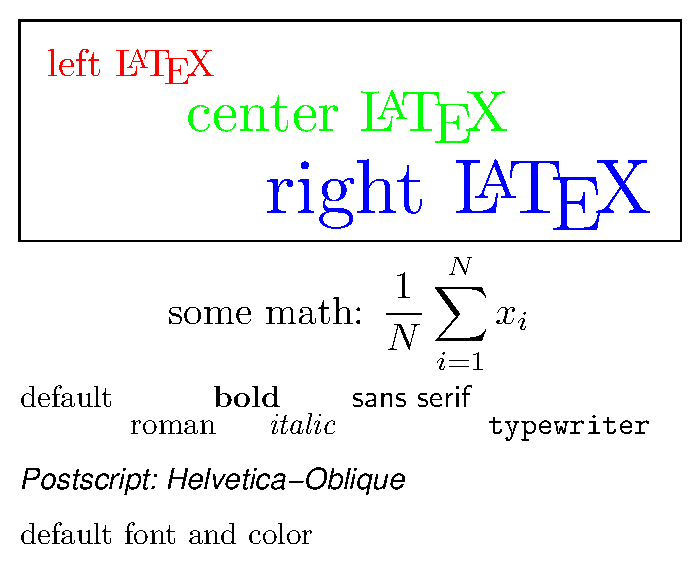
\includegraphics[width=0.5\textwidth]{figuras/test.eps}
	\caption[Esquema do banco de dados do \starlight.]
	{Esquema do banco de dados do \starlight.}
	\label{fig:EsquemaBDStarlight}
\end{figure}

\subsection{Amostra do \STARLIGHT}
\label{sec:Crossmatch:AmostraStarlight}

A amostra de galáxias do \starlight contém $926246$ espectros do \SDSS. A
identificação de cada espectro é feita através de um tripleto: a data juliana
média da observação ({\tt MJD}, {\em Mean Julian Date}), a identificação da
placa de suporte das fibras ópticas ({\tt Plate}) e a identificacão da fibra
utilizada para a obtenção do espectro ({\tt FiberID}). Este tripleto ({\tt MJD},
{\tt Plate}, {\tt FiberID}) identifica unicamente um espectro. Porém, é mais
conveniente (e eficiente) ter um identificador único (uma chave
primária\footnote{Chave primária é um conjunto de um ou mais campos tais que a
combinação de todos os campos da chave não se repete.}) para os registros num
banco de dados. No caso do \SDSS, a tabela de espectros ({\tt SpecObjAll}) tem
um identificador chamado {\tt SpecObjID}.

% TODO: Adicionar figura - esquema simplificado da BD do SDSS.
\begin{figure}
	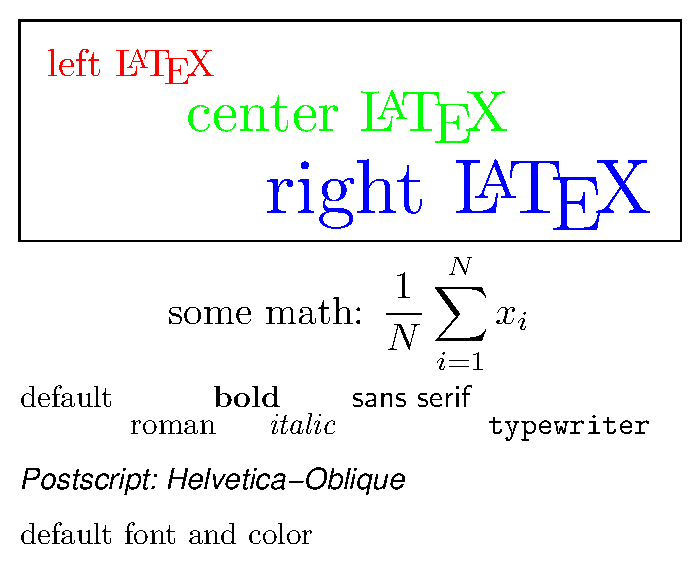
\includegraphics[width=0.5\textwidth]{figuras/test.eps}
	\caption[Esquema simplificado do banco de dados do \SDSS.]
	{Esquema simplificado do banco de dados do \SDSS.}
	\label{fig:EsquemaSDSS}
\end{figure}

Além de espectros, o banco de dados do \SDSS (figura \ref{fig:EsquemaSDSS})
contém fotometria de $1/4$ do céu. Os objetos com dados de fotometria
também tem um identificador único, {\tt ObjID}. Existe uma coluna na tabela de
espectros chamada {\tt BestObjID}, que aponta para o registro de fotometria
(tabela {\tt PhotoObjAll}) mais provável para cada espectro. É importante
salientar que nem todo espectro tem um {\tt BestObjID} definido.

A tabela de índices da amostra de galáxias do \starlight (esquema na figura
\ref{fig:TabelaAmostraStarlight}) contém inicialmente os tripletos [{\tt MJD},
{\tt Plate}, {\tt FiberID}]. Dentro do ambiente {CasJobs} do \SDSS
DR7\footnote{{\em CasJobs} \SDSS DR7 - \url{http://casjobs.sdss.org/CasJobs/}} a
tabela tem os valores de {\tt SpecObjID} e {\tt BestObjID} preenchida através da
execução da {\em query} mostrada na figura \ref{fig:AtualizaObjIds}. Entre os
objetos na amostra do \starlight, $622$ objetos não tem a sua contrapartida
fotométrica.

% TODO: Adicionar figura - Tabela amostra do starlight.
\begin{figure}
	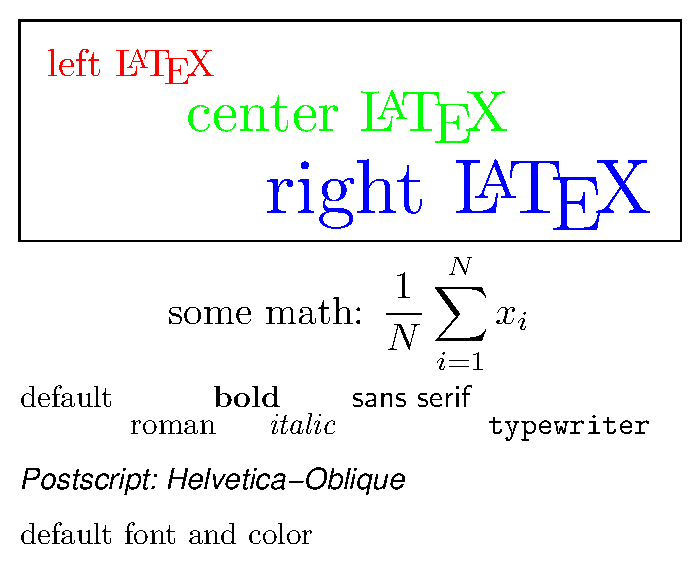
\includegraphics[width=0.5\textwidth]{figuras/test.eps}
	\caption[Tabela de índices da amostra do \starlight.]
	{Esquema da tabela de índices da amostra do \starlight. Os tipos de dados são
	referentes à implementação do banco de dados.}
	\label{fig:TabelaAmostraStarlight}
\end{figure}


%***************************************************************%
%                                                               %
%                   Crossmatch - SDSS X GALEX                   %
%                                                               %
%***************************************************************%

\section{Crossmatch \SDSS/\galex}

A identificação mútua ({\em crossmatch}) de objetos em {\em surveys} diferentes
é um problema razoavelmente complicado. A cobertura do céu de cada {\em survey}
em geral não é a mesma. Por outro lado, os objetos presentes em um {\em survey}
podem não ter sido detectados no outro. A probabilidade de duas fontes em
catálogos diferentes corresponderem a um mesmo objeto pode ser calculada como
função da separação entre elas e a precisão astrométrica das medidas
\citep{Budavari2008}.

\subsection{Identificação dos objetos}
\label{sec:Crossmatch:SDSSGalex:Identificacao}

\citet{Budavari2009} aplicam este método probabilístico ao \SDSS e ao \galex. O
{\em crossmatch} espacial é feito dentro de um RDMS (MSSQL, o mesmo usado no
{\em CasJobs}), utilizando técnicas avançadas de indexação \citep{Kunszt2000}. A
tabela resultante é uma relação ``muitos para muitos'', onde a maioria dos
objetos \galex tem apenas um objeto \SDSS associado, mas outras associações
podem ocorrer. Um exemplo onde pode ocorrer uma associação ``um para muitos'' é
o caso onde existe uma fonte fraca em UV (presente no \SDSS mas não detectada
pelo \galex) próxima a uma fonte presente tanto no UV quanto no óptico. O
algoritmo irá apontar estes dois objetos no \SDSS como candidatos a serem a
contrapartida óptica do objeto detectado no \galex. O caso inverso implicaria
numa associação ``muitos para um''. Nas tabelas \ref{tab:SDSSxGalexMatchesAIS} e
\ref{tab:SDSSxGalexMatchesMIS} há a quantidade de identificações para cada tipo
de associação, referentes aos {\em surveys} AIS e MIS, respectivamente. Os
valores foram determinados para o {\em crossmatch} entre \SDSS DR7 e \galex GR6,
disponível no {\em CasJobs} do \galex\footnote{{\em CasJobs} do \galex:
\url{http://galex.stsci.edu/casjobs/}}). O artigo citado acima mostra a mesma
tabela, com os resultados para dados do \SDSS DR6 e \galex GR3. A técnica
utilizada por \citeauthor{Budavari2009} agora faz parte do {\em pipeline} do
\galex. A distribuição do {\em CasJobs} inclui as ferramentas necessárias para
fazer o {\em crossmatch} espacial entre bancos de dados.

\begin{table}
	\caption[Identificações entre \SDSS DR7 e {\em survey} AIS do \galex GR6.]
	{Número de identificações entre \SDSS DR7 e {\em survey} AIS do \galex GR6, por
	associação.}
	\setlength{\tabcolsep}{1cm}
	\begin{tabular}{r r r r}
		\galex &          \multicolumn{3}{c}{\SDSS} \\
		\midrule
		       &          1 &         2 &    Muitos \\
		1      & 15.267.818 & 9.150.919 & 4.623.197 \\
		2      &  4.524.337 & 2.504.786 & 1.162.463 \\
		Muitos &    770.645 &   426.691 &   184.680 \\
	\end{tabular}
	\label{tab:SDSSxGalexMatchesAIS}
\end{table}

\begin{table}
	\caption[Identificações entre \SDSS DR7 e {\em survey} AIS do \galex GR6.]
	{Número de identificações entre \SDSS DR7 e {\em survey} MIS do \galex GR6, por
	associação.}
	\setlength{\tabcolsep}{1cm}
	\begin{tabular}{r r r r}
		\galex &         \multicolumn{3}{c}{\SDSS} \\
		\midrule
		       &         1 &         2 &    Muitos \\
		1      & 8.201.735 & 5.923.551 & 3.775.187 \\
		2      & 2.120.174 & 1.580.701 &   984.067 \\
		Muitos &   276.447 &   234.016 &   150.894 \\
	\end{tabular}
	\label{tab:SDSSxGalexMatchesMIS}
\end{table}


%***************************************************************%
%                                                               %
%      Crossmatch - Definição da amostra Starlight/GALEX        %
%                                                               %
%***************************************************************%

\section{Definição das amostras \SDSS/\STARLIGHT e \galex}
\label{sec:Crossmatch:DefAmostras}

\subsection{Relação de {\em crossmatch} entre \SDSS e \galex}
Como comentado na seção \ref{sec:Crossmatch:SDSSGalex:Identificacao}, no banco
de dados do \galex há uma tabela de {\em crossmatch} entre os objetos do \galex
e os seus correspondentes ópticos no catálogo do \SDSS, chamada {\tt xSDSSDR7}.
A descrição completa dos campos pode ser vista na tabela
\ref{tab:CamposXSDSSDR7}. Dado que a identificação não é necessariamente
unívoca, existem informações extras nesta tabela a fim de facilitar a seleção
dos melhores candidatos: {\tt DistanceRank} e {\tt MultipleMatchCount}.

A identificação cruzada também é feita na direção oposta. Dado um objeto do
\SDSS, foram encontrados os objetos do \galex candidatos. Para um par [{\tt
ObjID}, {\tt SDSSObjID}], há também os campos {\tt ReverseDistanceRank} e {\tt
ReverseMultipleMatchCount}.

\begin{table}
	\caption[Descrição dos campos da tabela {\tt xSDSSDR7}.]
	{Descrição dos campos da tabela {\tt xSDSSDR7}.}
	\begin{tabular}{l p{8cm}}
		Campo & Descrição\\
		\midrule
		{\tt ObjID} &
		Identificador único de objeto do \galex.
		\\
		{\tt SDSSObjID} &
		Identificador único do \SDSS.
		\\
		{\tt Distance} &
		Separação angular em segundos de arco.
		\\
		{\tt DistanceRank} &
		Um número inteiro, onde o valor $1$ indica que o objeto do \galex é o
		mais próximo do objeto \SDSS, o valor $2$ indica que ele é o segundo mais
		próximo, etc.
		\\
		{\tt ReverseDistanceRank} &
		Um número inteiro, onde o valor $1$ indica que o objeto do \SDSS é o mais
		próximo do objeto \galex, o valor $2$ indica que ele é o segundo mais
		próximo, etc.
		\\
		{\tt MultipleMatchCount} &
		Um número inteiro indicando quantos objetos \SDSS foram encontrados para o
		objeto \galex dentro do raio de busca.
		\\
		{\tt ReverseMultipleMatchCount} &
		Um número inteiro indicando quantos objetos \galex foram encontrados para o
		objeto \SDSS dentro do raio de busca.
		\\
	\end{tabular}
	\label{tab:CamposXSDSSDR7}
\end{table}

\subsection{Obtendo dados UV da amostra do \STARLIGHT}

A amostra do \starlight obtida na seção \ref{sec:Crossmatch:AmostraStarlight}
contém o identificador do catálogo de fotometria do \SDSS. Este identificador é
o mesmo utilizado na tabela {\tt XSDSSDR7}. A {\em query} da figura
\ref{fig:QueryMatchAIS} preenche a tabela chamada {\tt galex\_ais} com todos os
objetos da amostra do \starlight, junto com suas respectivas magnitudes NUV
({\tt FUV\_mag}) e FUV ({\tt NUV\_mag}), o erro na medida das magnitudes ({\tt
FUV\_magErr} e {\tt NUV\_magErr}), o tempo de exposição em cada filtro ({\tt
fexptime} e {\tt nexptime}), o índice de cor $E(B-V)$ ({\tt e\_bv}, ver seção
\ref{sec:Crossmatch:Correcoes}) e a distância entre a detecção do objeto
no \galex e no \SDSS ({\tt distance}). Esta tabela é esparsamente populada, com
um registro para cada objeto do \starlight, e os dados UV preenchidos somente
para os objetos com identificação positiva. Caso o objeto não tenha um
correspodente \galex, os valores serão nulos\footnote{Numa tabela, quando um
campo de um registro não possui valor definido, seu valor é dito ``nulo''. Em
SQL, a palavra-chave que representa um valor nulo é ``{\em null}''}. De forma
similar, os dados UV para o {\em survey} MIS foram armazenados na tabela {\tt
galex\_mis}.

A {\em query} mostrada na figura \ref{fig:QuerySampleAIS} monta a amostra a ser
utilizada no capítulo seguinte. As colunas selecionadas são as magnitudes
$ugriz$ do \SDSS, as magnitudes $FUV$ e $NUV$ do \galex e alguns parâmetros
físicos do \starlight (tabela \ref{tab:ParamFisicos}. Foram selecionadas também
informações sobre as linhas de emissão H$_\alpha$, H$_\beta$, [OIII](5007\AA) e
[NII](6584\AA). Foram montadas duas amostras, uma para o AIS e outra para o MIS.

\begin{table}
	\caption[Parâmetros físicos das galáxias utilizados na amostra.]
	{Parâmetros físicos das galáxias, obtidos do \starlight.}
	\begin{tabular}{l l}
		Coluna & Descrição \\
		\midrule
		{\tt mcor\_gal} & Logaritmo da massa estelar \\
		{\tt at\_flux}  & Logaritmo da idade média ponderada em fluxo \\
		{\tt at\_mass}  & Logaritmo da idade média ponderada em massa \\
		{\tt am\_flux}  & Metalicidade média ponderada em fluxo \\
		{\tt am\_mass}  & Metalicidade média ponderada em massa \\
		{\tt AV}       & Extinção causada por poeira (magnitude) \\
	\end{tabular}
	\label{tab:ParamFisicos}
\end{table}

\subsection{Completeza dos dados}

Foram escolhidos apenas identificações cruzadas do tipo um-para-um, ou seja, com
{\tt multipleMatchCount} e {\tt reverseMultipleMatchCount} iguais a $1$. Em
situações diferentes desta, caso houvesse mais de um candidato para uma mesma
deteção, seria necessária uma análise mais detalhada. Desta forma, optou-se por
uma confiabilidade maior nos dados utilizando apenas identificações unívocas, em
troca de uma amostra menor.

Outro artefato importante é que apenas um objeto foi escolhido, indepente do
{\em survey} \galex utilizado. Se existe um correspondente AIS e outro MIS para
o mesmo objeto da amostra, apenas o mais próximo é considerado.\fixme
% FIXME: Rever o critério de escolha dos matches simultaneos AIS e MIS.

% TODO: Alguma estatística.
TODO: Alguma estatística.


\section{Correções na fotometria UV}
\label{sec:Crossmatch:Correcoes}

\subsection{Poeira}
\label{sec:Crossmatch:Correcoes:Poeira}

% TODO: Correção por poeira etc.
Correção de poeira, \#comofas?

Catálogo do \galex provê os valores de índice de cor das galáxias com base no
modelo de \citet{Schlegel1998} para a poeira interestelar.

A correção é feita usando a CCM \citep{Cardelli1989}.
%a_FUV = 8.29 * ebv
%a_NUV = 8.18 * ebv
%CCM, Schlegel.

Ver seção 2.2.2 da tese do Abilio.

$$
	A_{FUV} = 8,29 E(B-V)
$$
$$
	A_{NUV} = 8,18 E(B-V)
$$

Foi feita a correção para magnitude absoluta usando KCORRECT de
\citet{Blanton2007}.


%% End of this chapter
